\section{Architecture}

The Solution architecture is decomposed into five main entities. 
\begin{description}
    \item[Device] IoT Environment Monitor, a Raspberry Pi 3 with Raspian Lite OS equipped with a sense hat sending telemetry to the server and getting device setting from server. The device application is implemented in Python 3.
    \item[Application] User Interface (UI) Application, an Angular 6 web app for telemetry monitoring and device management.
    \item[MQTT Broker] Publish/Subscribe Communication Middleware that handles communication between IoT Devices and the Server.
    \item[Server] Rest API, node.js server, encapsulating business logic and exposes services through HTTP endpoints and MQTT communication with devices.
    \item[Database] NoSQL Database, MongoDb, storing sensor telemetry and device twins 
\end{description}
Figure \ref{fig:arc} presents a model of the architecture.

\begin{figure}[H]
    \centering
    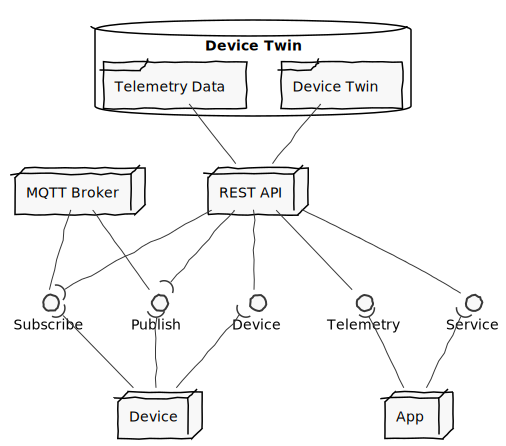
\includegraphics[width=0.7\textwidth]{out/figures/uml/architecture/architecture.png}
    \caption{Solution architecture as a deployment diagram with interfaces}
    \label{fig:arc}
\end{figure}

In the following section will the implementation and design consideration for each entity be explained. 